\section{Auswertung}
Die Auswertung, genauer die Fehlerrechnung, die Plots und Ausgleichsrechnung erfolgt mit den Paketen
Numpy \cite{numpy}, Uncertainties \cite{uncertainties}, Matplotlib \cite{matplotlib} und Scipy \cite{scipy} in der Programmiersprache python.
\subsection{Fehlerrechnung}
Zu Beginn der Auswertung sei gesagt, dass eine Ungenauigkeit von $\SI{10}{\percent}$ des analogen zum digitalen Glühkathodenvakuummessgeräts
bei der Messung festgestellt und im Folgenden berücksichtigt wurde.
Für das Pirani-Messgerät ist eine Ungenauigkeit von $\SI{30}{\percent}$ angegeben\cite{anleitung}.
Das Prinani-Messgerät ist das Modell Thermovac TR2005 von Leybold-Heraeus; die Heißkathode Ionivac IM210 ebenso von Leybold-Heraeus.

Auch muss erwähnt werden, dass die Zeitmessung mit einer Handystoppuhr erfolgte und eine durch menschliche Reaktion verursachte
Verzögerung von $\SI{180}{ms}$ beachtet wird\cite{reaktion}.
In den nachfolgenden Messwerttabellen sind die Abweichungen schon als einseitiger Fehler auf die Messzeit addiert.\\

Die Messungen


Die Mittelwerte werden nach
\begin{equation}
	\bar{x}=\frac{1}{N}\sum_{i}^N x_i
\end{equation}
und deren Standardabweichung mit
\begin{equation}
	\sigma_{\bar{x}} = \sqrt{\frac{1}{N(N-1)} \sum_{i}^N (x_i-\bar{x})^2}
\end{equation}
berechnet.
Für die Fehlerfortpflanzung einer Variablen $x_i$ gilt
\begin{equation}
	\sigma = \sqrt{\sum_{i}^N \Bigl(\frac{\partial f}{\partial x_i} \sigma_{x_i}\Bigr)^2}.
	\label{eq:gaussfehler}
\end{equation}
Für die Berechnung des Logarithmus für die Evakuierungsmessung muss der Fehler dessen aus bereits fehlerbehafteten Größen nach
\begin{equation}
	\sigma = \sqrt{\frac{\sigma_p^2}{(p-p_E)^2}+\frac{\sigma_{p0}^2}{(p_0-p_E)^2}+\sigma_{p_E}^2\bigl(\frac{1}{p_0-p_E}-\frac{1}{p_-p_E}\bigr)^2}
\end{equation}
berechnet werden.
\subsection{Bestimmung des Volumens}
Für die folgende Auswertung ist es unumgänglich, das Volumen des Messaufbaus zu bestimmen.
Tabelle $\ref{tab:Bauteile}$ zeigt, aufgelistet nach Pumpen- und Messart die verwendeten Bauteile und ihre Volumina.
Es wird zwischen der Evakuierungsmessung mit der Turbopumpe TE, derselben Messart mit der Drehschieberpumpe DE und der Leckratenmessung
mit der Drehschieberpumpe DL und mit der Turbopumpe TL unterschieden.\newline

\begin{table}[!hht]
	\centering
	\begin{tabular}{|c|c|c|c|c|c|c|}
		\hline
		Bauteil Nr. & Bauteilbezeichnung & {$\symup{Volumen} \:/\: l$}& TE & TL & DE & DL\\ \hline
		1	&	Tank & $9,5 \pm 0,8$ & 1 & 1 & 1 & 1 \\ \hline
		2	&	langer Schlauch & $0,8 \pm 0,1$ &  &  & 1 & 1 \\	\hline
		3	&	kurzer Schlauch & $0,087 \pm 0,011$ &  &  & 1 & 1 \\	\hline
		4a	&	T-Stück, klein & $0,013 \pm 0,002$ &  &  & 1 & 1 \\	\hline
		4b	&	T-Stück, groß & $0,25 \pm 0,01$ & 1 & 1 & 1 & 1 \\	\hline
		5a	&	Kreuzstück, klein & $0,016 \pm 0,002$ &  &  & 1 & 1 \\	\hline
		5b	&	Kreuzstück, groß & $0,177 \pm 0,09$ & 1 & 1 & 1 & 1 \\	\hline
		6a	&	Handventil 1, offen & $0,015 \pm 0,002$ &  & 1 & 1 & 2 \\	\hline
		6b	&	Handventil 1, geschlossen & $0,005 \pm 0,001$ &  2 & 1 & 2 & 1 \\	\hline
		7a	&	Handventil 2, offen & $0,025 \pm 0,005$ &  &  & 1 &  \\	\hline
		7b	&	Handventil 2, geschlossen & $0,0125 \pm 0,0025$ &  &  &  & 1 \\	\hline
		8a	&	Klappenventil, offen & $0,044 \pm 0,004$ & 1 &  &  &  \\	\hline
		8b	&	Klappenventil, geschlossen & $0,022 \pm 0,002$ &  & 1 & 1 & 1 \\	\hline
		9	&	Querschnittsverengung & $0,067 \pm 0,004$ & 1 &  &  &  \\	\hline
	\end{tabular}
	\caption{Auflistung der Bauteile.\cite{anleitung}}
	\label{tab:Bauteile}
\end{table}
Die Teilvolumina der jeweiligen Aufbauten werden addiert und im Folgenden angegeben. Die Fehlerberechnung erfolgt mit Formel $\ref{eq:gaussfehler}$.
Es ergeben sich
\begin{align*}
   V_\text{TE}=&\SI{10,0 \pm 0,8}{l}\\
   V_\text{TL}=&\SI{10,0 \pm 0,8}{l}\\
   V_\text{DE}=&\SI{10,9 \pm 0,8}{l}\\
   V_\text{DL}=&\SI{10,9 \pm 0,8}{l}.
\end{align*}

\subsection{Turbomolekularpumpe}
Für die Turbomolekularpumpe werden im Folgenden beide Messverfahren ausgewertet.
Zum anschließenden Vergleich sind folgende Herstellerangaben\cite{anleitung} gegeben:\\
Turbo SST81 der Firma ILMAC mit einem Saugvermögen von $\SI{77}{l/s}$
\subsubsection{Evakuierungsmessung}
\begin{table}[H]
\tiny
\centering
\begin{tabular}{c|c|c|c|c|c|c|c|c|c|c}
{$p \:/\: \si{mbar}$} & {$\ln{\Bigl( \frac{p(t)-p_E}{p_0-p_E}\Bigr)}$} & {$t_1 \:/\: \si{s} $} & {$t_2 \:/\: \si{s}$} & {$t_3 \:/\: \si{s}$} & {$t_4 \:/\: \si{s}$} & {$t_5 \:/\: \si{s}$} & {$t_6 \:/\: \si{s}$}& {$t_7 \:/\: \si{s}$} & {$t_8 \:/\: \si{s}$} & {$\bar{t} \:/\: \si{s}$}\\
\midrule
$(8,1 \pm \, 0,8)\cdot 10^{-3}$ & 0 \pm 0,4 & 0 &  0 & 0 & 0 & 0 & 0 & 0 & 0 & 0\\
$(6,0 \pm \, 0,6)\cdot 10^{-3}$ & $-(0,29 \pm \, 0,15)$ & 0,44 & 0,87 & 0,78 & 0,70 & 0,79 & 0,87 & 0,78 & 0,83 & $0,76 \pm \, 0,05$\\
$(3,0 \pm \, 0,3)\cdot 10^{-3}$ & $-(0,98 \pm \, 0,15)$ & 0,74 & 1,40 & 1,21 & 1,09 & 1,35 & 1,43 & 1,41 & 1,62 & $1,28 \pm \, 0,10$\\
$(6,0 \pm \, 0,6)\cdot 10^{-4}$ & $-(2,62 \pm \, 0,15)$ & 2,82 & 3,13 & 2,82 & 3,00 & 3,10 & 3,20 & 3,09 & 2,79 & $3,00 \pm \, 0,06$\\
$(3,0 \pm \, 0,3)\cdot 10^{-4}$ & $-(3,34 \pm \, 0,16)$ & 4,01 & 4,04 & 3,99 & 3,87 & 3,93 & 4,02 & 3,93 & 4,03 & $3,94 \pm \, 0,13$\\
$(6,0 \pm \, 0,6)\cdot 10^{-5}$ & $-(5,20 \pm \, 0,19)$ & 6,52 & 6,86 & 6,61 & 7,04 & 6,44 & 6,72 & 6,71 & 6,70 & $6,70 \pm \, 0,07$\\
$(3,0 \pm \, 0,3)\cdot 10^{-5}$ & $-(6,35 \pm \, 0,27)$ & 10,14 & 10,03 & 10,00 & 9,44 & 10,29 & 9,42 & 9,06 & 8,94 & $9,67 \pm \, 0,21$\\
$(1,6 \pm \, 0,2)\cdot 10^{-5}$ & - & - &  -& -& -& -& -& -& -& - \\
\end{tabular}
\caption{Messwerte für die Evakuierungskurve der Turbomolekularpumpe.}
\label{tab:EvakuierungskurveTurbo}
\end{table}

\begin{figure}[H]
  \centering
  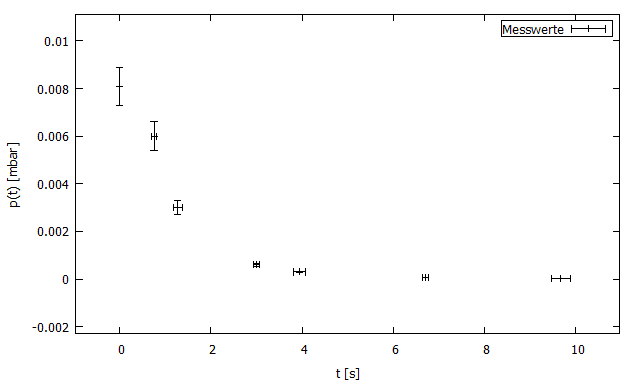
\includegraphics[width=14cm]{bilder/thefinalfinalplot.png}
  \caption{Exponentielle Darstellung der Evakuierungskurve der Turbomolekularpumpe.}
  \label{turboexponential}
\end{figure}

\begin{figure}[H]
  \centering
  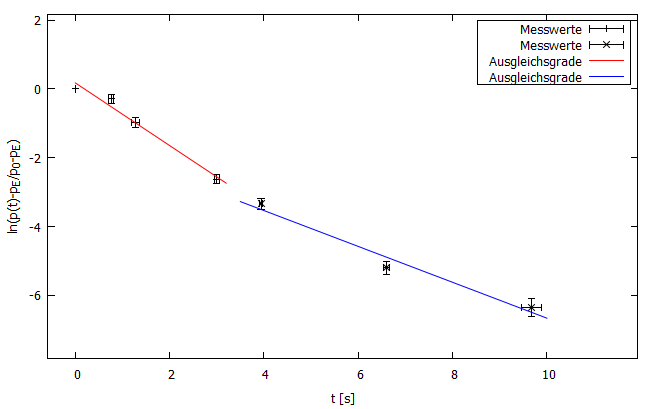
\includegraphics[width=14cm]{bilder/turbodruckplot.png}
  \caption{Logarithmische Darstellung der Evakuierungskurve der Turbomolekularpumpe.}
  \label{turboplot}
\end{figure}
Abbildung $\ref{turboexponential}$ zeigt die Messwerte aus Tabelle $\ref{tab:EvakuierungskurveTurbo}$ aufgetragen.
Es zeigt sich ein exponentieller Zusammenhang.
In der logarithmischen Darstellung (Abbildung $\ref{turboplot}$) wurden die Messwerte unterteilt und zwei lineare Ausgleichsrechnungen durchgeführt, da für die unterschiedlichen Druckbereiche das Saugvermögen nicht konstant ist.
Die Ausgleichsgeraden haben die Form
\begin{equation}
 h(x)=mx+b.
\end{equation}
Aus den Regressionsparametern wird das Saugvermögen durch $S=-mV$ bestimmt.\\

Bereich 1: $8 \cdot 10^{-3} \, \si{mbar} \geq p \geq 6 \cdot 10^{-4} \, \si{mbar}$\\
\begin{align*}
	m_1=& -\SI{0,91 \pm 0,09}{1/s}\\
	b_1=& \si{0,18 \pm 0,16}\\
	S_1=& \SI{9,1 \pm 1,2}{l/s}
\end{align*}
Bereich 2: $6 \cdot 10^{-4} \, \si{mbar} \geq p \geq 3 \cdot 10^{-5} \, \si{mbar}$\\
\begin{align*}
	m_2=& -\SI{0,52 \pm 0,09}{1/s}\\
	b_2=& -\si{1,45 \pm 0,66}\\
	S_2=& \SI{5,2 \pm 1,0}{l/s}
\end{align*}

\subsubsection{Leckratenmessung}
Die folgenden Tabellen $\ref{tab:leck_Turbo1}$, $\ref{tab:leck_Turbo2}$, $\ref{tab:leck_Turbo3}$ und $\ref{tab:leck_Turbo4}$ zeigen die Messwerte zur Leckratenmessung der Turbomolekularpumpe.

\begin{table}[H]
\centering
\begin{tabular}{c|c|c|c|c}
	{$p \:/\: \si{mbar}$} & {$t_1 \:/\: \si{s} $} & {$t_2 \:/\: \si{s} $} & {$t_3 \:/\: \si{s} $} & {$\bar{t} \:/\: \si{s}$}\\
\midrule
$(5,0 \pm \, 0,5)\cdot 10^{-5}$ &0 &0 &0 &0\\
$(8,0 \pm \, 0,8)\cdot 10^{-5}$ &   0,32 &  0,66 &  0,39 & $0,46 \pm 0,11$\\
$(2,0 \pm \, 0,2)\cdot 10^{-4}$ &   1,71  &  1,83 &  1,65 & $1,73 \pm 0,06$\\
$(4,0 \pm \, 0,4)\cdot 10^{-4}$ &   5,91 &  6,02 &  6,40 & $6,11 \pm 0,15$\\
$(8,0 \pm \, 0,8)\cdot 10^{-4}$ &   13,05 &  13,14 &  14,02 & $13,40 \pm 0,31$\\
$(2,0 \pm \, 0,2)\cdot 10^{-3}$ &   34,01 &  34,50 &  36,37 & $34,96 \pm 0,77$\\
$(4,0 \pm \, 0,4)\cdot 10^{-3}$ &  61,18 & 62,18 & 66,18 & $63,18 \pm 1,53$\\
\end{tabular}
\caption{Gleichgewichtsdruck bei $p_G=(5,0 \pm \, 0,5)\cdot 10^{-5} \, \si{mbar}$.}
\label{tab:leck_Turbo1}
\end{table}

\begin{table}[H]
\centering
\begin{tabular}{c|c|c|c|c}
	{$p \:/\: \si{mbar}$} & {$t_1 \:/\: \si{s} $} & {$t_2 \:/\: \si{s} $} & {$t_3 \:/\: \si{s} $} & {$\bar{t} \:/\: \si{s}$}\\
\midrule
$(10 \pm \, 1)\cdot 10^{-5}$ &0 &0 &0 &0\\
$(3,0 \pm \, 0,3)\cdot 10^{-4}$ &   1,22 &  0,96 &  0,70 & $0,96 \pm 0,16$\\
$(6,0 \pm \, 0,6)\cdot 10^{-4}$ &   3,00  &  2,77 &  2,69 & $2,82 \pm 0,10 $\\
$(9,0 \pm \, 0,9)\cdot 10^{-4}$ &   4,85 &  4,56 &  4,47 & $4,63 \pm 0,12 $\\
$(2,0 \pm \, 0,2)\cdot 10^{-3}$ &   10,88 &  10,78 &  11,30 & $11,00 \pm 0,14 $\\
$(4,0 \pm \, 0,4)\cdot 10^{-3}$ &   20,09 &  20,00 &  19,61 & $19,90 \pm 0,15 $\\
$(6,0 \pm \, 0,6)\cdot 10^{-3}$ &  28,26 & 27,78 & 27,36 & $27,80 \pm 0,26 $\\
\end{tabular}
\caption{Gleichgewichtsdruck bei $p_G=(1,0 \pm \, 0,1)\cdot 10^{-5} \, \si{mbar}$.}
\label{tab:leck_Turbo2}
\end{table}

\begin{table}[H]
\centering
\begin{tabular}{c|c|c|c|c}
	{$p \:/\: \si{mbar}$} & {$t_1 \:/\: \si{s} $} & {$t_2 \:/\: \si{s} $} & {$t_3 \:/\: \si{s} $} & {$\bar{t} \:/\: \si{s}$}\\
\midrule
$(1,5 \pm \, 0,2)\cdot 10^{-5}$ &0 &0 &0 &0\\
$(3,0 \pm \, 0,3)\cdot 10^{-4}$ &   0,57 &  0,40 &  0,40 & $0,46 \pm 0,06$\\
$(6,0 \pm \, 0,6)\cdot 10^{-4}$ &   1,27  &  1,36 &  1,40 & $1,34 \pm 0,04$\\
$(9,0 \pm \, 0,9)\cdot 10^{-4}$ &   2,71 &  2,55 &  2,48 & $2,58 \pm 0,07$\\
$(2,0 \pm \, 0,2)\cdot 10^{-3}$ &   6,70 &  6,31 &  6,22 & $6,41 \pm 0,15$\\
$(4,0 \pm \, 0,4)\cdot 10^{-3}$ &   12,30 &  11,94 &  11,89 & $12,04 \pm 0,13$\\
$(6,0 \pm \, 0,6)\cdot 10^{-3}$ &  17,37 & 17,31 & 17,10 & $17,26 \pm 0,08$\\
\end{tabular}
\caption{Gleichgewichtsdruck bei $p_G=(1,5 \pm \, 0,2)\cdot 10^{-4} \, \si{mbar}$.}
\label{tab:leck_Turbo3}
\end{table}

\begin{table}[H]
\centering
\begin{tabular}{c|c|c|c|c}
	{$p \:/\: \si{mbar}$} & {$t_1 \:/\: \si{s} $} & {$t_2 \:/\: \si{s} $} & {$t_3 \:/\: \si{s} $} & {$\bar{t} \:/\: \si{s}$}\\
\midrule
$(2,0 \pm \, 0,2)\cdot 10^{-4}$ &0 &0 &0 &0\\
$(5,0 \pm \, 0,5)\cdot 10^{-4}$ &   0,64 &  0,82 &  0,74 & $0,73 \pm 0,06$\\
$(8,0 \pm \, 0,8)\cdot 10^{-4}$ &   1,57  &  1,83 &  1,65 & $1,68 \pm 0,08$\\
$(2,0 \pm \, 0,2)\cdot 10^{-3}$ &   4,76 &  4,69 &  5,04 & $4,83 \pm 0,11$\\
$(4,0 \pm \, 0,4)\cdot 10^{-3}$ &   9,57 &  9,77 &  9,71 & $9,68 \pm 0,06$\\
$(6,0 \pm \, 0,6)\cdot 10^{-3}$ &   13,67 &  13,94 &  13,78 & $13,80 \pm 0,08$\\
$(8,0 \pm \, 0,8)\cdot 10^{-3}$ &  17,50 & 17,87 & 17,59 & $17,65 \pm 0,12$\\
\end{tabular}
\caption{Gleichgewichtsdruck bei $p_G=(2,0 \pm \, 0,2)\cdot 10^{-4} \, \si{mbar}$.}
\label{tab:leck_Turbo4}
\end{table}
Die Daten aus den vorheringen Tabellen sind in den Abbildungen $\ref{leckrate1}$, $\ref{leckrate2}$, $\ref{leckrate3}$ und $\ref{leckrate4}$ graphisch dargestellt.
\begin{figure}[H]
  \centering
  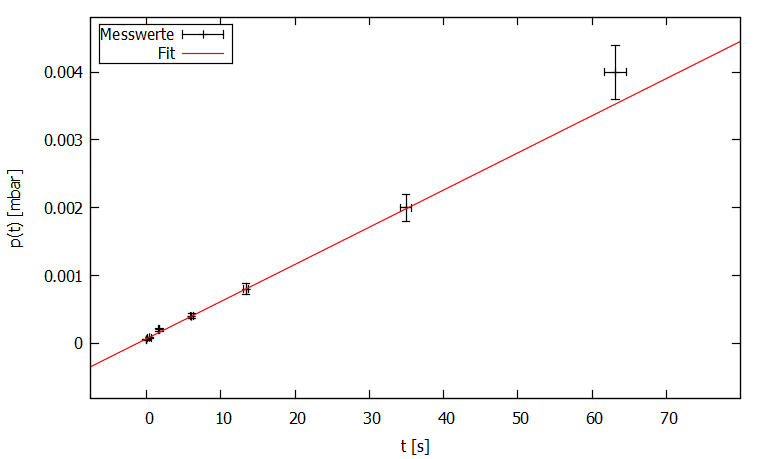
\includegraphics[width=14cm]{bilder/leckratefit1.png}
  \caption{Graphische Darstellung der Leckratenmessung der Turbomolekularpumpe für $p_G=(5,0 \pm \, 0,5)\cdot 10^{-5} \, \si{mbar}$.}
  \label{leckrate1}
\end{figure}
\begin{figure}[H]
  \centering
  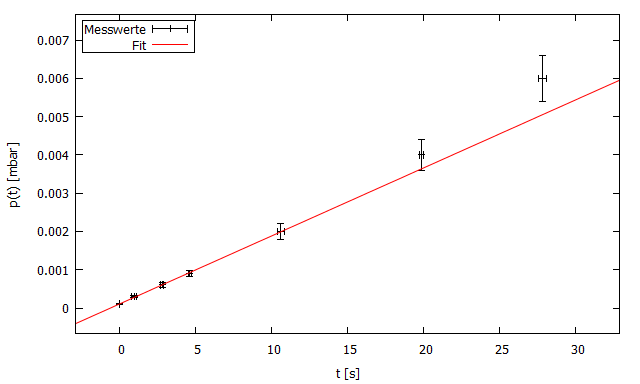
\includegraphics[width=14cm]{bilder/leckratefit2.png}
	\caption{Graphische Darstellung der Leckratenmessung der Turbomolekularpumpe für $p_G=(1,0 \pm \, 0,1)\cdot 10^{-5} \, \si{mbar}$.}
  \label{leckrate2}
\end{figure}
\begin{figure}[H]
  \centering
  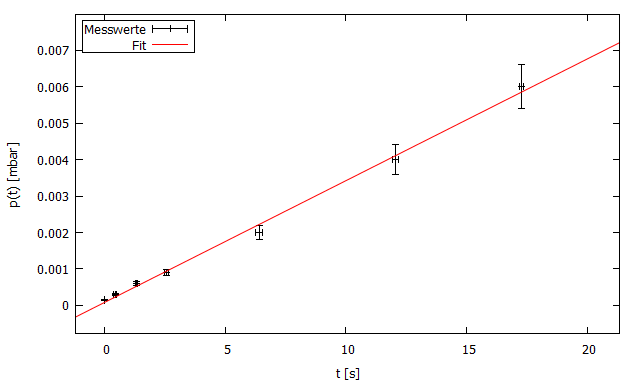
\includegraphics[width=14cm]{bilder/leckratefit3.png}
	\caption{Graphische Darstellung der Leckratenmessung der Turbomolekularpumpe für $p_G=(1,5 \pm \, 0,2)\cdot 10^{-4} \, \si{mbar}$.}
  \label{leckrate3}
\end{figure}
\begin{figure}[H]
  \centering
  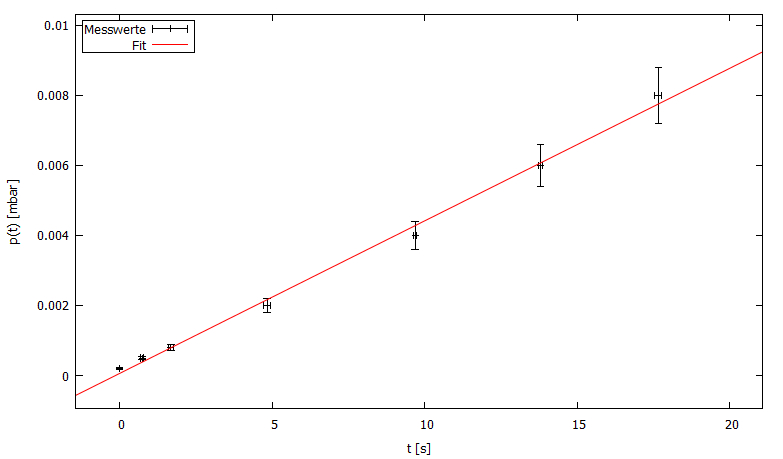
\includegraphics[width=14cm]{bilder/leckratefit4.png}
	\caption{Graphische Darstellung der Leckratenmessung der Turbomolekularpumpe für $p_G=(2,0 \pm \, 0,2)\cdot 10^{-4} \, \si{mbar}$.}
  \label{leckrate4}
\end{figure}
Auch hierfür wurde eine lineare Ausgleichsrechnung der Form
\begin{equation}
	h(x)=mx+b
\end{equation}
durchgeführt.
Aus den Zusammenhängen $\ref{eq:leckrate1}$ und $\ref{eq:leckrate2}$ und dem Steigungsparameter $m$ wird mit $S=\frac{V}{p_G}m$
das Saugvermögen $S$ berechnet.\\

Abbildung $\ref{leckrate1}$:
	\begin{align*}
		p_G=& (5,0 \pm \, 0,5)\cdot 10^{-5} \, \si{mbar}\\
		m_1=& (6,13 \pm 0,17)\cdot 10^{-5} \, \si{mbar/s}\\
		b_1=& (3 \pm 5)\cdot 10^{-5} \, \si{mbar}\\
		S_1=& \SI{12,3 \pm 1,6}{l/s}
	\end{align*}
	Abbildung $\ref{leckrate2}$:
		\begin{align*}
			p_G=& (10 \pm \, 1)\cdot 10^{-5} \, \si{mbar}\\
			m_2=& (1,86 \pm 0,07)\cdot 10^{-4} \, \si{mbar/s}\\
			b_2=& (9,9 \pm 0,8)\cdot 10^{-4} \, \si{mbar}\\
			S_2=& \SI{18,6 \pm 2,5}{l/s}
		\end{align*}
		Abbildung $\ref{leckrate3}$:
			\begin{align*}
				p_G=& (1,5 \pm \, 0,2)\cdot 10^{-4} \, \si{mbar}\\
				m_3=& (3,34 \pm 0,09)\cdot 10^{-4} \, \si{mbar/s}\\
				b_3=& (7,87 \pm 7,30)\cdot 10^{-5} \, \si{mbar}\\
				S_3=& \SI{22,3 \pm 3,6}{l/s}
			\end{align*}
		Abbildung $\ref{leckrate4}$:
			\begin{align*}
				p_G=& (2,0 \pm \, 0,2)\cdot 10^{-4} \, \si{mbar}\\
				m_4=& (4,4 \pm \, 0,2)\cdot 10^{-4} \, \si{mbar/s}\\
				b_4=& (0,6 \pm \, 1,1)\cdot 10^{-4} \, \si{mbar}\\
				S_4=& \SI{22 \pm 3}{l/s}
			\end{align*}

\subsection{Drehschieberpumpe}
Ebenso für die Drehschieberpumpe folgt die Auswertung mit anschließendem Vergleich mit der
Herstellerangabe\cite{anleitung}:\\
Drehschieber Pfeiffer Duo 004A mit einem Saugvermögen von $\SI{1,1}{l/s}$\newpage
Die folgende Tabelle zeigt die Messwerte zur Bestimmung der Evakuierungskurve.
\subsubsection{Evakuierungsmessung}
\begin{table}[H]
\centering
\begin{tabular}{c|c|c|c|c|c|c|c}
{$p \:/\: \si{mbar}$} & {$\ln{\Bigl( \frac{p(t)-p_E}{p_0-p_E}\Bigr)}$} & {$t_1 \:/\: \si{s} $} & {$t_2 \:/\: \si{s}$} & {$t_3 \:/\: \si{s}$} & {$t_4 \:/\: \si{s}$} & {$t_5 \:/\: \si{s}$} & {$\bar{t} \:/\: \si{s}$}\\
\midrule
$(1000 \pm \, 300)$ & 0 \pm 0,4 & 0 &  0 & 0 & 0 & 0 & 0\\
$(100 \pm \, 30)$ & -(2,3 \pm \, 0,4) & 18,62 & 11,59 & 16,47 & 15,02 & 16,43 & $15,63 \pm \, 1,17$\\
$(40 \pm \, 12)$ & -(3,2 \pm \, 0,4) & 35,33 & 26,49 & 32,97 & 34,34 & 33,50 & $32,53 \pm \, 1,57$\\
$(10 \pm \, 3)$ & -(4,6 \pm \, 0,4) & 49,85 & 42,19 & 49,28 & 48,84 & 49,01 & $47,83 \pm \, 1,42$\\
$(6 \pm \, 1,8)$ & -(5,1 \pm \, 0,4) & 54,99 & 46,42 & 54,25 & 54,31 & 54,18 & $52,83 \pm \, 1,61$\\
$(4 \pm \, 1,2)$ & -(5,5 \pm \, 0,4) & 59,42 & 50,29 & 57,74 & 57,65 & 58,36 & $56,69 \pm \, 1,62$\\
$(2 \pm \, 0,6)$ & -(6,2 \pm \, 0,4) & 65,83 & 57,38 & 64,60 & 64,50 & 64,79 & $63,42 \pm \, 1,53$\\
$(1 \pm \, 0,3)$ & -(6,9 \pm \, 0,4) & 73,00 & 64,02 & 71,62 & 69,82 & 71,97 & $70,09 \pm \, 1,80$\\
$(0,6 \pm \, 0,18)$ & -(7,5 \pm \, 0,4) & 79,54 & 70,73 & 77,92 & 77,80 & 78,18 & $76,8 \pm \, 1,56$\\
$(0,4 \pm \, 0,12)$ & -(7,9 \pm \, 0,4) & 86,35 & 77,33 & 85,30 & 85,24 & 85,19 & $83,9 \pm \, 1,65$\\
$(0,2 \pm \, 0,06)$ & -(8,7 \pm \, 0,5) & 99,69 & 90,02 & 98,98 & 98,17 & 98,83 & $97,14 \pm \, 1,80$\\
$(0,1 \pm \, 0,03)$ & -(9,7 \pm \, 0,6) & 111,79 & 101,65 & 110,30 & 111,17 & 111,87 & $109,36 \pm \, 1,95$\\
$(0,06 \pm \, 0,02)$ & -(10,8 \pm \, 1,2) & 125,13 & 113,88 & 128,72 & 129,62 & 130,60 & $125,59 \pm \, 3,07$\\
$(0,04 \pm \, 0,01)$ & - & - & - & - & - & - & -
\end{tabular}
\caption{Messwerte für die Evakuierungskurve der Drehschieberpumpe.}
\label{tab:EvakuierungskurveDreh}
\end{table}



Je nach Druckbereich, wird der Graph unterteilt und gesonderte lineare Fits erstellt.
Es folgt die graphische Darstellung der logarithmierten Werte aus Tabelle $\ref{tab:EvakuierungskurveDreh}$.

\begin{figure}[H]
  \centering
  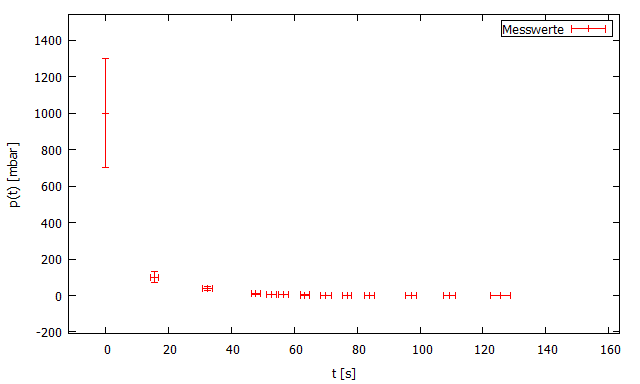
\includegraphics[width=14cm]{bilder/drehexpo.png}
  \caption{Exponentielle Darstellung der Evakuierungskurve der Drehschieberpumpe.}
  \label{expoevakuierungdreh}
\end{figure}
\begin{figure}[H]
  \centering
  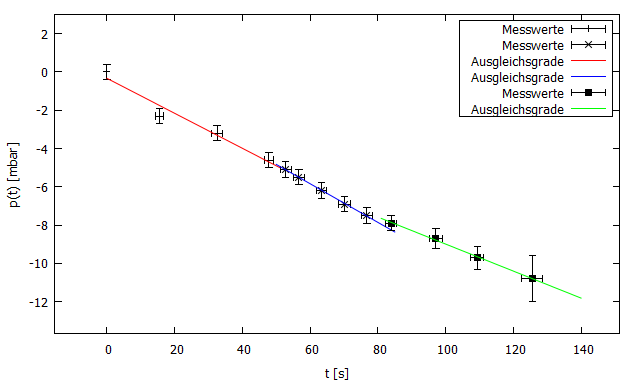
\includegraphics[width=14cm]{bilder/evakuierungDreh.png}
  \caption{Logarithmische Darstellung der Evakuierungskurve der Drehschieberpumpe.}
  \label{evakuierungdreh}
\end{figure}

Für die drei Bereiche wurden lineare Ausgleichsgeraden der Form
\begin{equation}
	h(x)=mx+b
\end{equation}
erstellt.\\
Durch die Regressionsberechnung ergeben sich folgende Parameter für die drei Bereiche und das daraus durch $S=-mV$ errechnete Saugvermögen:\\
Bereich 1: $\SI{1000}{mbar} \geq p \geq \SI{10}{mbar}$\\
\begin{align*}
	m_1=& -\SI{0,09 \pm 0,02}{1/s}\\
	b_1=& -\si{0,33 \pm 0,39}\\
	S_1=& \SI{0,98 \pm 0,23}{l/s}
\end{align*}
Bereich 2: $\SI{10}{mbar} \geq p \geq \SI{0,6}{mbar}$\\
\begin{align*}
	m_2=& -\SI{0,100 \pm 0,002}{1/s}\\
	b_2=& \si{0,22 \pm 0,11}\\
	S_2=& \SI{1,09 \pm 0,09}{l/s}
\end{align*}
Bereich 3: $\SI{0,6}{mbar} \geq p \geq \SI{0,06}{mbar}$\\
\begin{align*}
	m_3=& -\SI{0,071 \pm 0,003}{1/s}\\
	b_3=& -\si{(1,93 \pm 0,27)}\\
	S_3=& \SI{0,77 \pm 0,07}{l/s}
\end{align*}

\subsubsection{Leckratenmessung}
Ebenso wie für die Turbopumpe auch, folgen zunächst die Messwerttabellen für die Leckratenmessung
unter den unterschiedlichen Gleichgewichtsdrücken $\ref{tab:leck_Dreh1}$, $\ref{tab:leck_Dreh2}$, $\ref{tab:leck_Dreh3}$ und $\ref{tab:leck_Dreh4}$.
\begin{table}[H]
\centering
\begin{tabular}{c|c|c|c|c}
	{$p \:/\: \si{mbar}$} & {$t_1 \:/\: \si{s} $} & {$t_2 \:/\: \si{s} $} & {$t_3 \:/\: \si{s} $} & {$\bar{t} \:/\: \si{s}$}\\
\midrule
$1,0 \pm \, 0,3$ &0 &0 &0 &0\\
$2,0 \pm \, 0,6$ &   8,53 &  8,91 &  8,75 & $8,73 \pm 0,11$\\
$4,0 \pm \, 1,2$ &   24,89  &  22,93 &  25,06 & $24,29 \pm 0,68 $\\
$6,0 \pm \, 1,8$ &   40,78 &  38,00 &  39,19 & $39,32 \pm 0,81 $\\
$10,0 \pm \, 3,0$ &   73,05 &  70,53 &  71,96 & $71,85 \pm 0,73 $\\
$20,0 \pm \, 6,0$ &   172,71 &  148,99 &  155,35 & $159,02 \pm 7,10 $\\
\end{tabular}
\caption{Gleichgewichtsdruck bei $p_G=(1,0 \pm \, 0,1)  \, \si{mbar}$.}
\label{tab:leck_Dreh1}
\end{table}

\begin{table}[H]
\centering
\begin{tabular}{c|c|c|c|c}
	{$p \:/\: \si{mbar}$} & {$t_1 \:/\: \si{s} $} & {$t_2 \:/\: \si{s} $} & {$t_3 \:/\: \si{s} $} & {$\bar{t} \:/\: \si{s}$}\\
\midrule
$0,80 \pm \, 0,24$ &0 &0 &0 &0\\
$1,0 \pm \, 0,3$ &   2,34 &  1,86 &  1,20 & $1,80 \pm 0,33$\\
$2,0 \pm \, 0,6$ &   13,42  &  12,23 &  11,76 & $12,47 \pm 0,50 $\\
$4,0 \pm \, 1,2$ &   32,99 &  31,52 &  32,01 & $32,17 \pm 0,43 $\\
$6,0 \pm \, 1,8$  &   50,15 &  50,65 &  49,51 & $50,10 \pm 0,33 $\\
$10,0 \pm \, 3,0$ &   88,14 &  90,21 &  90,73 & $89,69 \pm 0,80 $\\
\end{tabular}
\caption{Gleichgewichtsdruck bei $p_G=(0,80 \pm \, 0,08) \, \si{mbar}$.}
\label{tab:leck_Dreh2}
\end{table}

\begin{table}[H]
\centering
\begin{tabular}{c|c|c|c|c}
	{$p \:/\: \si{mbar}$} & {$t_1 \:/\: \si{s} $} & {$t_2 \:/\: \si{s} $} & {$t_3 \:/\: \si{s} $} & {$\bar{t} \:/\: \si{s}$}\\
\midrule
$0,40 \pm \, 0,12$ &0 &0 &0 &0\\
$0,60 \pm \, 0,18$ &   4,26 &  4,72 &  4,45 & $4,48 \pm 0,13$\\
$1,0 \pm \, 0,3$ &   16,84  &  17,05 &  17,29 & $17,06 \pm 0,13 $\\
$2,0 \pm \, 0,6$ &   45,09 &  43,40 &  44,21 & $44,23 \pm 0,49 $\\
$4,0 \pm \, 1,2$ &   93,98 &  90,09 & 90,21 & $91,43 \pm 1,28 $\\
$6,0 \pm \, 1,8$ &   132,43 &  131,15 &  133,37 & $132,32 \pm 0,64 $\\
\end{tabular}
\caption{Gleichgewichtsdruck bei $p_G=(0,40 \pm \, 0,04) \, \si{mbar}$.}
\label{tab:leck_Dreh3}
\end{table}

\begin{table}[H]
\centering
\begin{tabular}{c|c|c|c|c}
	{$p \:/\: \si{mbar}$} & {$t_1 \:/\: \si{s} $} & {$t_2 \:/\: \si{s} $} & {$t_3 \:/\: \si{s} $} & {$\bar{t} \:/\: \si{s}$}\\
\midrule
$0,10 \pm \, 0,03$ &0 &0 &0 &0\\
$0,15 \pm \, 0,05$ &   1,91 &  1,99 &  1,52 & $(1,81 \pm 0,15)$\\
$0,20 \pm \, 0,06$ &   7,70  &  8,64 &  8,67 & $(8,34 \pm 0,32) $\\
$0,30 \pm \, 0,09$ &   18,89 &  21,62 &  19,79 & $(20,10 \pm 0,49) $\\
$0,40 \pm \, 0,12$ &   45,77 &  46,39 & 43,27 & $(45,14 \pm 0,80) $\\
$0,60 \pm \, 0,18$ &   95,86 &  92,23 &  94,75 & $(94,28 \pm 1,07) $\\
\end{tabular}
\caption{Gleichgewichtsdruck bei $p_G=(0,10 \pm \, 0,01) \, \si{mbar}$.}
\label{tab:leck_Dreh4}
\end{table}
Anschließend lassen sich die graphischen Darstellungen in den Abbildungen $\ref{leckdreh1}$, $\ref{leckdreh2}$, $\ref{leckdreh3}$ und $\ref{leckdreh4}$ finden.
\begin{figure}[H]
  \centering
  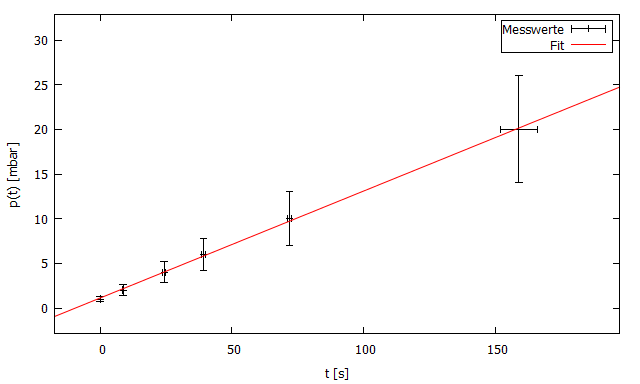
\includegraphics[width=14cm]{bilder/leckdrehfit1.png}
	\caption{Graphische Darstellung der Leckratenmessung der Drehschieberpumpe für $p_G=(1,0 \pm \, 0,3)  \, \si{mbar}$.}
  \label{leckdreh1}
\end{figure}
\begin{figure}[H]
  \centering
  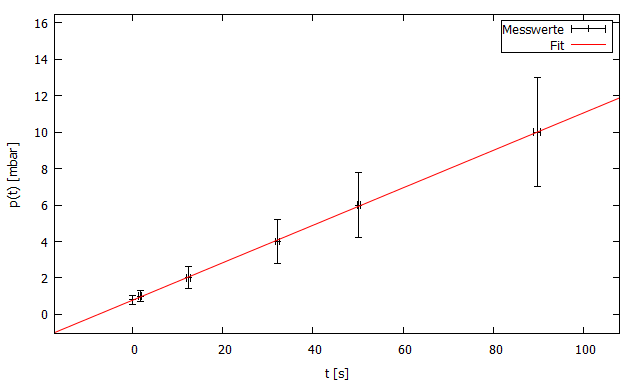
\includegraphics[width=14cm]{bilder/leckdrehfit2.png}
	\caption{Graphische Darstellung der Leckratenmessung der Drehschieberpumpe für $p_G=(0,80 \pm \, 0,24) \, \si{mbar}$.}
  \label{leckdreh2}
\end{figure}
\begin{figure}[H]
  \centering
  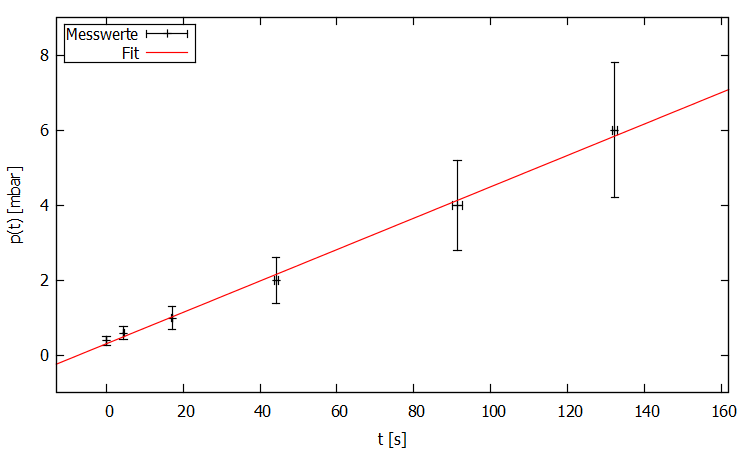
\includegraphics[width=14cm]{bilder/leckdrehfit3.png}
	\caption{Graphische Darstellung der Leckratenmessung der Drehschieberpumpe für $p_G=(0,40 \pm \, 0,12) \, \si{mbar}$.}
  \label{leckdreh3}
\end{figure}
\begin{figure}[H]
  \centering
  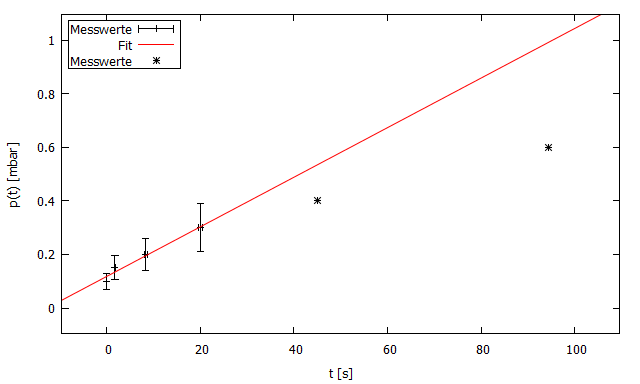
\includegraphics[width=14cm]{bilder/leckdrehfit4.png}
	\caption{Graphische Darstellung der Leckratenmessung der Drehschieberpumpe für $p_G=(0,10 \pm \, 0,03) \, \si{mbar}$.}
  \label{leckdreh4}
\end{figure}
Die Regressionsgeraden besitzen dieselbe lineare Form wie bei der Leckratenmessung der Turbopumpe auch und so lässt sich ebenso das Saugvermögen
aus dem Steigungsparameter $m$ und dem Volumen $V$ mit $S=\frac{V}{p_G}m$ unter den verschiedenen Gleichgewichtsdrücken $p_G$ berechnen.\\
Abbildung $\ref{leckdreh1}$:
	\begin{align*}
		p_G=& (1,0 \pm \, 0,3)  \, \si{mbar}\\
		m_1=& (0,12 \pm 0,002) \, \si{mbar/s}\\
		b_1=& (1,11 \pm 0,12) \, \si{mbar}\\
		S_1=& \SI{1,31 \pm 0,41}{l/s}
	\end{align*}
	Abbildung $\ref{leckdreh2}$:
		\begin{align*}
			p_G=& (0,80 \pm \, 0,24) \, \si{mbar}\\
			m_2=& (0,103 \pm 0,001) \, \si{mbar/s}\\
			b_2=& (0,77 \pm 0,04) \, \si{mbar}\\
			S_2=& \SI{1,36 \pm 0,44}{l/s}
		\end{align*}
		Abbildung $\ref{leckdreh3}$:
			\begin{align*}
				p_G=& (0,40 \pm \, 0,12) \, \si{mbar}\\
				m_3=& (0,0418 \pm 0,0013)\, \si{mbar/s}\\
				b_3=& (0,31 \pm 0,08) \, \si{mbar}\\
				S_3=& \SI{1,09 \pm 0,36}{l/s}
			\end{align*}
		Abbildung $\ref{leckdreh4}$:
			\begin{align*}
				p_G=& (0,10 \pm \, 0,03) \, \si{mbar}\\
				m_4=& (0,009 \pm \, 0,001) \, \si{mbar/s}\\
				b_4=& (0,12 \pm \, 0,02) \, \si{mbar}\\
				S_4=& \SI{0,98 \pm 0,33}{l/s}
			\end{align*}
